\documentclass[10pt,letterpaper]{article}
\usepackage[utf8]{inputenc}
\usepackage{amsmath}
\usepackage{amsfonts}
\usepackage{amssymb}
\usepackage{graphicx}

\begin{document}
\section*{CEL Team VI - Demonstration Plan Overview}
\begin{figure}
	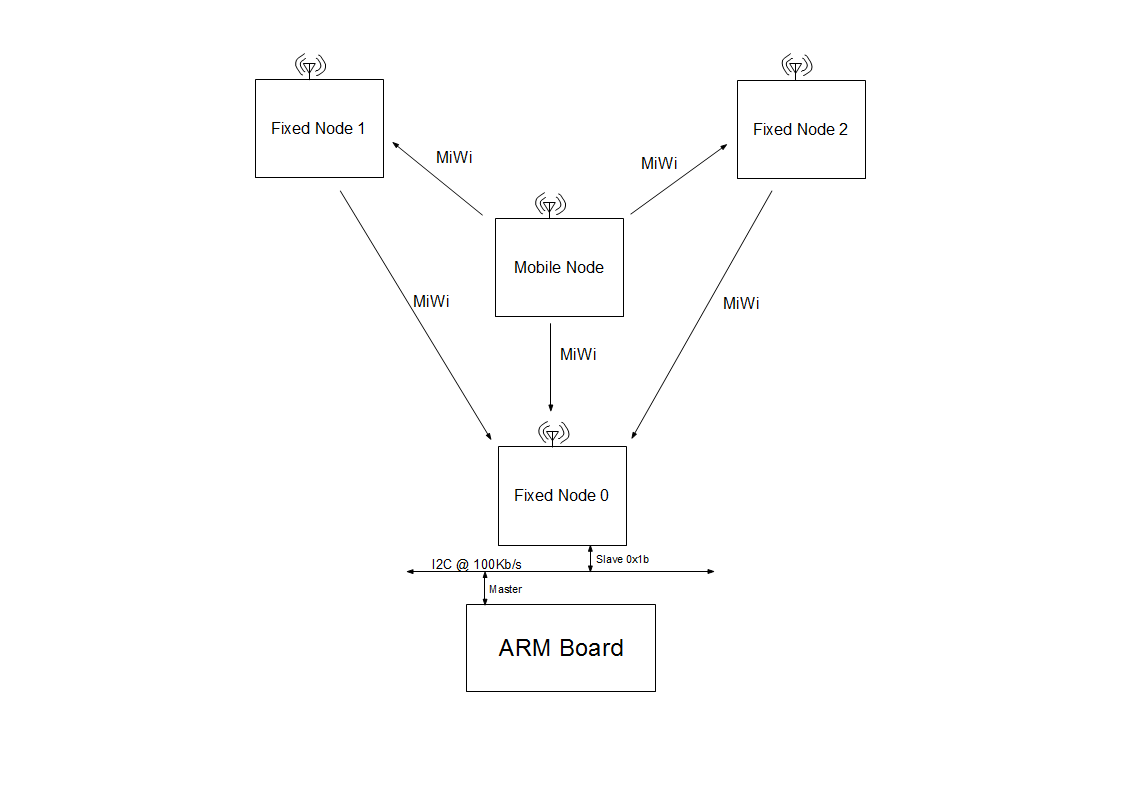
\includegraphics[scale=0.5]{Overall_Poster_BD.png}
	\caption{System Diagram}
\end{figure}
\subsection*{System Overview}
\paragraph*{}
This system performs wireless position sensing using an 802.15.4 \textit{MiWi} network.  The \textit{MiWi} transceivers have limited range with a maximum
power output of about 1 mW.  Several fixed transceivers are positioned in the sensing area to receive beacon packets from a mobile transmitter.  The mobile
transmitter beacons eight times per second with GPS data from its on-board receiver.
\paragraph*{}
Each fixed transceiver calculates the received signal strength (RSSI) of the incoming packets and forwards the RSSI information to all other fixed nodes.  Connected
to one fixed node is an ARM processor board.  This board uses the known location of the fixed nodes, and their RSSI information to estimate the position of the
mobile transmitter.
\paragraph*{}
The Universal Transverse Mercator (UTM) system is used for this system.  It allows for a localize projection of the earth's ellipsoid onto a 2D coordinate system.  After
following a gradient descent algorithm to estimate the transmitter position, two range and bearing calculations are performed.  First, the range and bearing from the ARM
board is calculated, then range and bearing (error) from the recorded GPS position is calculated.  Additionally both GPS and calculated positions are displayed on the LCD,
recorded to a storage device, and displayed on a dynamic webpage.
\section*{Demonstration Plan}
\begin{enumerate}
\item Demonstrate communication and parsing of GPS data by entering receiver node calibration mode.
	\begin{enumerate}
	\item The User interfaces with the ARM LCD screen and follows on-screen calibration instructions.
	\item GPS data is received over UART on the mobile node.  \textit{Verification: DVS3100 Logic Analyzer}
	\item GPS data is then parsed and transmitted using MiWi to the receivers. \textit{Verification: MIWI\_STATUS and MIWI\_TX LEDs}
	\item ARM board queries node0 for GPS position information. \textit{Verification: DVS3100 Logic Analyzer }
	\item ARM board accumulates several samples of GPS position information and determines the designated node's position. \textit{Verification: Current DMS GPS Position is displayed during calibration.}
	\end{enumerate}
\item Demonstrate position estimation algorithm by placing the system into run mode.
	\begin{enumerate}
	\item As the user moves about, GPS data is transmitted from the mobile node.
	\item Each receiver node calculates received signal strength from the mobile node.
	\item node1 and node2 forward their received signal strength to node0.
	\item ARM board queries node0 for all RSSI and GPS data. \textit{Verification: DVS3100 Logic Analyzer}
	\item Positioning algorithm updates position estimation based on RSSI data. \textit{Verification: Position information on LCD Display}
	\end{enumerate}
\item Demonstrate web interface functionality
	\begin{enumerate}
	\item After section 2 is complete, continue to operate system in run mode.
	\item Establish a connection to the ARM webserver.
	\item Recent position information will be displayed on the web page.
	\item The web page refresh rate is once every two seconds.
	\end{enumerate}
\item Demonstrate filesystem functionality
	\begin{enumerate}
	\item After sections 2 and 3 are complete, shut down the ARM board.
	\item Remove the SD card and insert into a computer.
	\item Display the logged information on a computer.
	\end{enumerate}
\item Demonstration Complete.
\end{enumerate}
\end{document}
